\chapter{Beslutning under usikkerhet}
\label{kap:beslutning} % Opprinnelig kapittelnr: 16

\section{Innledning}

En beslutningstaker skal treffe en beslutning under usikkerhet.
Skjematisk tenker vi oss at problemet kan beskrives slik

\begin{table}[h] \centering
\begin{tabular}{c|c|cccc}
      &               & \multicolumn{4}{c}{Beslutninger} \\
Utfall&Sannsynligheter& $a_1$&$a_2$&$\cdots$&$a_n$ \\ \hline
 $u_1$ & $p_1$ & $g_{11}$ & $g_{12}$ & $\cdots$ & $g_{1n}$ \\
 $u_2$ & $p_2$ & $g_{21}$ & $g_{22}$ & $\cdots$ & $g_{2n}$ \\
 $\vdots$& $\vdots$& $\vdots$& $\vdots$&   & $\vdots$ \\
 $u_m$ & $p_m$ & $g_{m1}$ & $g_{m2}$ & $\cdots$ & $g_{mn}$ \\ \hline
\end{tabular}\\[1mm]
\caption{Beslutningstabell}
\label{tab:beslutningstabell} % Tabell_1
\end{table}
Her foreligger $n$ mulige beslutninger (aksjoner) $a_1, a_2, \ldots, a_n$
og beslutningstakeren må velge en av disse.  Konsekvensene av
den valgte beslutning avhenger av hvilket av de $m$ utfallene
$u_1, u_2, \ldots, u_m$ som inntreffer.  I tabellen betegner $p_i$
sannsynligheten for utfallet $u_i$, mens $g_{ij}$ gir uttrykk for
konsekvensen dersom utfallet $u_i$ inntreffer og beslutningstakeren har
valgt beslutning $a_j$, i mange forbindelser er det hensiktsmessig å
kalle $g_{ij}$'ene for gevinster.

Eksempler på beslutningsproblemer som skjematisk kan beskrives slik
er mange, la oss nevne noen få:

\begin{itemize}
\item  Hasardspill, f.eks. med en eller flere terninger.  Utfallene er
       de ulike kombinasjoner av øyne, og beslutningene er hvilken
       av disse kombinasjoner som det satses på og eventuelt hvor mye.
\item  Et visst kvantum av en vare skal innkjøpes til lager for
       senere salg.  Etterspørselen er usikker og utfallene 
       representerer ulike mulige etterspurte kvanta, og beslutningene
       er de ulike kvanta som kan kjøpes inn for lager.
\item  Et prosjekt skal gjennomføres og utfallene er de ulike forløp
       av hele prosjektperioden, og beslutningene representerer
       handlingsprogrammer, dvs. en beskrivelse av hvordan en skal
       forholde seg til enhver situasjon som kan oppstå i 
       prosjektperioden.
\end{itemize}
Usikkerheten i et beslutningsproblem kan være av varierende karakter.
På den ene side kan den bestå i ren tilfeldighet, slik tilfellet
ofte er i hasardspill.  På den annen side har vi problemer der
usikkerheten består i manglende informasjon om tingenes tilstand,
eksempelvis dersom man vurderer å ta med noen hjem til middag, uten
å vite om man har de nødvendige ingredienser for en vellykket
aften.  I det første tilfellet kan sannsynligheter for de ulike 
utfall fastsettes noenlunde objektivt, i det andre ikke, en kan stille
spørsmål om det i det hele tatt er rimelig å gjøre bruk av
sannsynligheter her.  Det finnes også problemer som inneholder
elementer av begge typer usikkerhet, eksempelvis dersom vi har en vare
på lager og vi kjenner etterspørselstilbøyeligheten, f.eks.
uttrykt ved en sannsynlighetsfordeling, men i tillegg er det usikkerhet
om hva konkurrentene gjør for å eventuelt øke sin markedsandel.

Konsekvensene for beslutningstakeren i et beslutningsproblem kan også
ha varierende karakter, fra rene økonomiske konsekvenser, til
konsekvenser av typen goodwill, trivsel for seg selv og eventuelt andre som
beslut\-nings\-takeren velger å ta omsyn til (f.eks. samfunnets tarv).
Økonomiske konsekvenser lar seg som regel tallfeste, mens andre 
konsekvenser lar seg vanskelig tallfeste, i hvert fall slik at de er
sammenlignbare og eventuelt kan oppsummeres i et enkelt tall.\\

\begin{eksempel}{Maskinforretning}
En maskinforretning vurderer å kjøpe inn et visst antall av en
bestemt landbruksmaskin til lager før sesongen.  Anta at bedriften
har valgt å beskrive problemet med følgende tabell.
\begin{center}
\begin{tabular}{c|c|rrrr}
Etter-     &    Sann-     & \multicolumn{4}{c}{Gevinster ved innkjøp}\\
spørsel &  synlighet   &       0  &  1  &  2  &  3 \\ \hline
   0       &   0.1        &       0  & $-$2  & $-$4  & $-$6 \\
   1       &   0.3        &      $-$1  &  5  &  3  &  1 \\
   2       &   0.4        &      $-$2  &  4  & 10  &  8 \\
   3       &   0.2        &      $-$3  &  3  &  9  & 15 \\ \hline
\end{tabular} 
\end{center}
Sannsynlighetene i tabellen er fastlagt ut fra vurdering av behov og 
øko\-no\-misk evne hos potensielle kunder, eventuelt også en vurdering
av konkurrenters engasjement.  Her er etterspurt kvantum høyst 3, 
med 2 som det mest sannsynlige.  Gevinstene i tabellen er fastlagt ut
fra en regnskapsmessig vurdering for de kommende år (enheten i
tabellen kan f.eks. være kr. 10 000).  Vi ser at hver solgt maskin 
bidrar med +5 til gevinsten, hver usolgt maskin med $-2$ (som skyldes 
lagerkostnader fram til neste sesong og eventuelt salg til lavere pris).
Tap av goodwill ved udekket etterspørsel bidrar med $-1$ pr. enhet.

La oss ta disse tallene for gitt og prøve å bestemme et fornuftig
inn\-kjøps\-kvan\-tum:  En mulig beslutning er å velge å kjøpe
inn det mest sannsynlige etterspurte kvantum, dvs. 2 enheter.  Dette
ignorerer helt konsekvensene.  En annen mulighet er å treffe den
beslutning som, for det verst (evt.best) tenkelige utfall for 
beslutningen, sikrer den største gevinst.  Her er dette å kjøpe
inn 1 (evt.3) enheter.  Dette ignorerer sannsynlighetene for de ulike
utfall, og vil nok bli ansett for å være for pessimistisk
(evt. for optimistisk).  I faglitteraturen blir disse to beslutningene
kalt henholdsvis {\em maximin og maximax} beslutningen.  I praksis
ønsker vi en beslutning som tar omsyn til både sannsynlighetene
og konsekvensene.  En mulighet er å beregne forventet gevinst for hver
beslutning.  Eksempelvis dersom det kjøpes inn 2 enheter blir
forventet gevinst
\[     EG = (-4) \cdot 0.1 + 3 \cdot 0.3 + 10 \cdot 0.4 + 9 \cdot 0.2 = 6.3 \]
og tilsvarende for de andre.  Vi får

\begin{center}
\begin{tabular}{l|cccc}
Innkjøpt kvantum    &      0     &     1     &     2     &     3 \\ \hline
Forventet gevinst      &   $-1.7$   &    3.5    &    6.3    &    5.9
\end{tabular}
\end{center}
Vi ser at den beslutning som gir størst forventet gevinst er å
kjøpe inn 2 enheter.
\end{eksempel}

Et eksempel som dette reiser en del prinsipielle spørsmål:

\begin{enumerate}
\item  Er det rimelig å bruke sannsynligheter til å beskrive ikke 
       bare rene tilfeldigheter, men også ukjente omstendigheter, 
       f.eks. andre personers bevisste men ukjente valg?
\item  Kan vi rettferdiggjøre bruk av et enkelt mål for 
       konsekvensene i form av gevinster?
\item  Er i så fall forventede gevinster et rimelig vurderingsgrunnlag
       for valg av beslutning?
\item  Hvordan kan vi sammenfatte separate vurderinger av en rekke 
       usikre momenter og separate vurderinger av en rekke ulike konsekvenser?
\end{enumerate}
Svarene på disse sp{\o{rsmål vil avhenge noe av karakteren av det
beslutningsproblem som foreligger.  En beskrivelse av beslutningsproblemer
som i Tabell~\ref{tab:beslutningstabell} kalles beskrivelse på {\em normalform}.  I praksis
vil en ofte foretrekke å beskrive problemet på såkalt
{\em ekstensiv form}.  Dette er emnet for de følgende avsnitt som
også inneholder delvise svar på spørsmålene ovenfor.


                                                   

\section{Beslutningsanalyse}

Vi vil ta opp en teknikk for beslutningsanalyse som har vist seg nyttig i
praksis, spesielt for kompliserte beslutningsproblemer av prosjekttypen,
der mange delavgjørelser må treffes over tid.  Teknikken kalles
{\em beslutningstreanalyse}, og vi illustrerer den best ved å 
gjennomdrøfte et noenlunde realistisk problem: 

Den 10.august 1996 får elektronikkfirmaet A/S Elektron vite at
A/S Kjemi trenger 1000 kontrollenheter av en bestemt type for installasjon
i en ny fabrikk.  A/S Kjemi har tidligere benyttet konvensjonelle enheter,
prisen på disse er nå 14 000 kr. pr. enhet.  A/S Elektron tror at de 
kan være i stand til å lage en kontrollenhet som er bedre enn
den eksisterende, og overveier å bygge en prototyp på egen
bekostning.  A/S Kjemi har sagt seg villig til å teste prototypen,
og dersom den viser seg å være bedre enn den konvensjonelle, så
vil firmaet plassere hele ordren på 1000 enheter hos A/S Elektron,
til pris 14 000 kr. pr. enhet.  Levering og oppgjør for partiet skal
finne sted 31.des. 1996.

A/S Elektron mener at kostnadene ved å utvikle prototypen er 
800 000 kr., og at dersom de får ordren, kan de tenke seg to 
produksjonsmetoder:

\begin{center}
\begin{tabular}{ll}
 Metode 1: & faste kostnader 1 200 000 kr. \\
           & variable kostnader 10 000 kr. pr. enhet.\\[1mm]
 Metode 2: & faste kostnader 1 700 000 kr. \\
           & variable kostnader 9 000 kr. pr. enhet.
\end{tabular}
\end{center}
Produksjonen etter metode 2 krever kjøp av en del tilleggsutstyr og 
leve\-rings\-datoen for dette er noe usikker.  A/S Elektron regner imidlertid
med at dersom de velger metode 2 og går til innkjøp av utstyret,
men dette ikke når fram til en fastsatt dato, kan de skifte over til
metode 1 og allikevel oppfylle kontrakten.  Vi regner med at de faste 
kostnader da blir 1 700 000 kr., dvs. tilleggsinvesteringen på
500 000 kr. ``går tapt".  Produksjonen av de 1000 enhetene vil delvis
gå på bekostning av A/S Elektrons øvrige virksomhet.  En 
hadde regnet med en netto inntekt på 1 000 000 kr. på andre
prosjekter i tiden fram til 31.des. 1996.  Dersom produksjon finner sted,
regner en med at denne inntekten blir halvert til 500 000 kr.  A/S Elektron
regner med at arbeidet med å utvikle prototypen ikke har slike
sidevirkninger.  Anta at A/S Elektron's ``status" den 10.aug. 1996 er\\
$-$1 000 000 kr.  Med status menes et mål for foretakets tilstand i
øyeblikket.  Det kan for eksempel være netto likvide aktiva. 
A/S Elektron regner med at sannsynligheten for at de skal få ordren
er 0.5, og at sannsynligheten for at bestilt tilleggsutstyr skal nå
fram i tide er 0.8.

Anta at A/S Elektron ønsker å maksimere forventet fortjeneste i 
pro\-sjekt\-perioden (fram til 31.des. 1996).  Som konsulenter skal vi 
bestemme et optimalt handlingsprogram for foretaket.

Dette er et eksempel på et beslutningsprogram under usikkerhet, av
sekvensiell natur, der den første beslutning får konsekvenser for
senere beslutninger.  Slike beslutningsproblemer lar seg ofte beskrive
oversiktlig ved et såkalt {\em beslutningstre}.  I Figur~\ref{fig:AS_Elektron} er det
vist hvordan et beslutningstre for vårt problem kan se ut.

\begin{figure}[ht]
\centering
 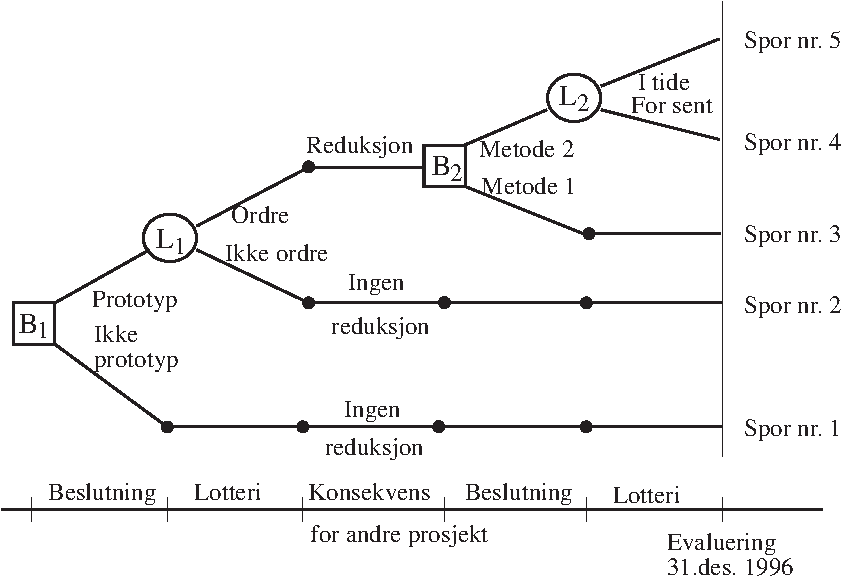
\includegraphics[scale=0.8]{figurer/fig16_1.pdf} 
\caption{Beslutningtre A/S Elektron}
	\label{fig:AS_Elektron}
\end{figure}
Vi tenker oss treet med roten på venstre side av arket med 
forgreninger mot høyre, hver gren mellom to forgreningspunkter svarer
enten til en beslutning eller et utfall av et \emph{``lotteri"}.  Vi har to
typer forgreningspunkter, markert med henholdsvis firkant og sirkel:

\begin{itemize}
\item betyr en beslutningssituasjon, hver gren som løper mot % HJS tok vekk [$\Box$]
      høyre fra dette forgreningspunktet svarer til en mulig beslutning.\\
\item[$\bigcirc$] betyr et lotteri, hver gren som løper mot høyre fra
      dette for\-gre\-nings\-punktet svarer til et mulig utfall av dette lotteriet.
\end{itemize}

Treet er organisert slik at beslutninger og utfall opptrer i logisk 
rekke\-følge, dvs. i den rekkefølge informasjonen blir tilgjengelig.
Ved et for\-grenings\-punkt har vi til rådighet all den informasjon som
ligger i grener som går forut for forgreningspunktet, dvs. grener
som kan nås ved å gå mot venstre langs grenene.

La oss forsøke å rettferdiggjøre treet i Figur~\ref{fig:AS_Elektron}: 
Firkanten $B_1$ helt til venstre betegner den initiale beslutningssituasjon:
skal foretaket utvikle en prototype eller ikke, svarende til henholdsvis
øvre og nedre gren ut fra firkanten.  Utvikles ikke prototypen er all
usikkerhet fjernet, og det er heller ikke flere beslutningsproblemer, vi
fører grenen fram til enden av treet (eva\-luerings\-datoen).  Velger en å
utvikle prototypen står en ovenfor et lotteri $L_1$ med to utfall:
ordre eller ikke ordre.  Dersom en ikke få ordren, blir det ikke flere
forgreninger, grenen føres fram til enden.  Dersom en får ordren,
er en i en ny beslutningssituasjon $B_2$, skal det produseres etter 
metode 1 eller metode 2. Velger en å produsere etter metode 1, er vi ved
enden av treet, men velges metode 2 er vi i lotterisituasjonen $L_2$:
blir det nødvendige tilleggs\-utstyret levert i tide eller ikke.  Vi ser
at prosjektet kan følge et av 5 ulike spor gjennom treet, et spor 
svarende til hvert av endepunktene nummerert fra 1 til 5.

\begin{figure}[ht]
\centering
 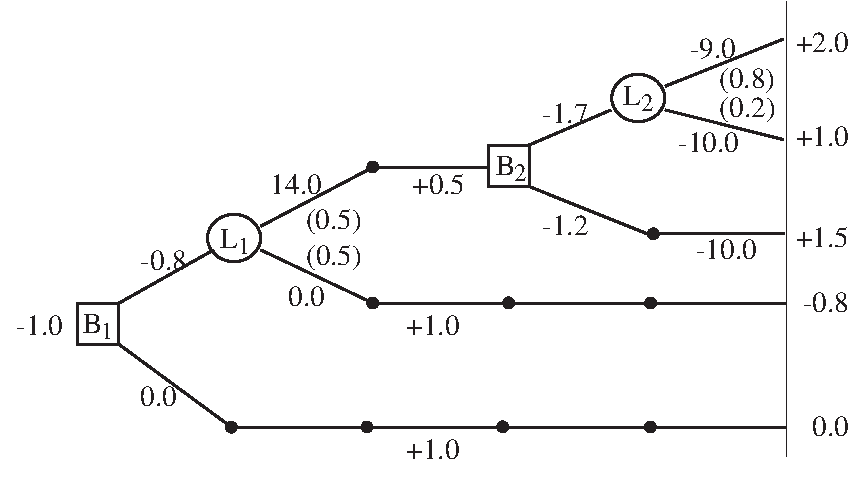
\includegraphics[scale=0.8]{figurer/fig16_2.pdf} 
\caption{Beslutningtre med data (Alle beløp i mill.)}
	\label{fig:alle_data}
\end{figure}

I Figur~\ref{fig:alle_data} er beslutningstreet påført alle de relevante data som er 
gitt i teksten.  Sannsynligheter er påført i parantes.  Ved starten
er status $-$1 000 000, og dersom en velger å utvikle en prototyp 
påløper kostnader 800 000.  Dersom en får ordren blir 
salgsinntekten av de ferdige enheter 14 000 000 og i tillegg kommer 
netto 500 000 fra andre prosjekter.  Produseres etter metode 1 påløper
faste kostnader 1 200 000 og variable kostnader 10 000 000.  For hvert spor
gjennom treet får vi en betalingsstrøm som gir en bestemt
fortjeneste, spor nr. 3 gir for eksempel
\begin{eqnarray*}
\mbox{Fortjeneste}&=&-800\;000+14\;000\;000+500\;000-1\;200\;000-10\;000\;000\\
                     &=&+2\;500\;000
\end{eqnarray*}
Status ved enden av treet = $-$1 000 000 +2 500 000 = 1 500 000.\\
For hvert av de fem endepunktene av treet er påført status ved 
prosjekt\-perio\-dens slutt. Det overlates til leser å sjekke alle detaljer.

Vi ser at spor nr.5 ville vært mest gunstig for foretaket, men dette 
kan ikke med sikkerhet realiseres, foretaket må først få 
ordren og tilleggsutstyret må nå fram i tide, og slik informasjon
foreligger ikke på det tidspunkt foretaket skal treffe sin initiale
beslutning.  Et handlingsprogram må inneholde regler om hvilken 
beslutning som skal treffes i enhver beslutningssituasjon som kan oppstå
i prosjektperioden.  Vi skal finne det handlingsprogram som maksimerer 
forventet fortjeneste i prosjektperioden, dvs. fram til enden av treet.
I dette tilfellet blir det ekvivalent med å maksimere forventet status
ved enden av treet.  Vi vil foretrekke å bruke dette begrep i den
videre diskusjon, bl.a. fordi dette gir et uttrykk for foretakets evne
til å inngå nye engasjementer ved prosjektperiodens slutt.

For å finne et handlingsprogram som er optimalt i den forstand vi har
definert, kan vi i hovedtrekk gjøre følgende:

\begin{enumerate}
\item Beregn foretakets status ved hvert av de fem endepunktene av treet.
\item Beregn systematisk ``verdien" av alle forgreningspunkter ved å 
      starte i endepunktene av treet som gis verdi lik status, og gå
      så baklengs i treet til roten.  Hver lotteriforgrening gis
      verdi lik forventet verdi av grenene, mens hver beslutningsforgrening
      får verdien til den gren som har størst verdi. Denne gren 
      beholdes, de andre strykes.
\item Et optimalt handlingsprogram finnes ved å starte ved roten, og
      følge de grener som ikke er strøket ut.
\end{enumerate}

\noindent Dette arbeidsprogram er utført i Figur~\ref{fig:analyse_tre}.
\begin{figure}[ht]
\centering
 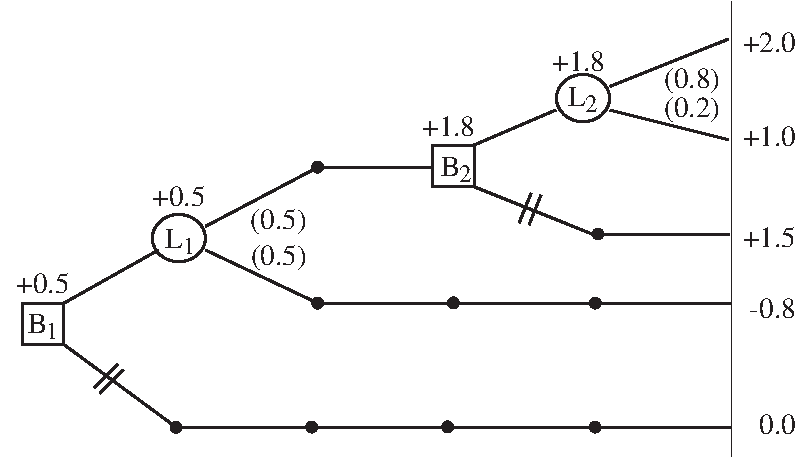
\includegraphics[scale=0.8]{figurer/fig16_3.pdf} 
\caption{Analyse av beslutningstre (Alle beløp i mill.)}
	\label{fig:analyse_tre}
\end{figure}

La oss illustrere hvordan beregningene utføres:\\
Figur~\ref{fig:lotteri} viser lotteriet $L_2$ som gir verdien +2 000 000 med sannsynlighet
0.8, verdien +1 000 000 med sannsynlighet 0.2.  Forventet verdi blir

       \[   0.8\cdot 2\;000\;000 + 0.2\cdot 1\;000\;000 = 1\;800\;000     \]
Når kriteriet er forventet sluttverdi, vil beslutningstakeren være
indifferent mellom dette lotteri og et sikkert beløp på
1 800 000. Vi kan derfor tildele forgreningspunktet $L_2$ verdien 
+1 800 000. Sett fra beslutningspunktet $B_2$ ser situasjonen nå ut 
som i Figur~\ref{fig:beslutning}.  
\begin{figure}[ht]
\centering
	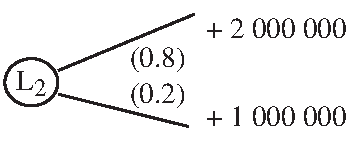
\includegraphics[scale=1.0]{figurer/fig16_4.pdf} 
\caption{Lotteri}
	\label{fig:lotteri}
\end{figure}
\begin{figure}[ht]
\centering
	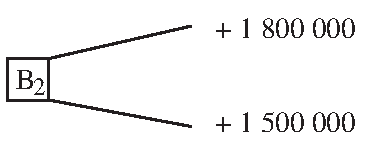
\includegraphics[scale=1.0]{figurer/fig16_5.pdf} 
\caption{Beslutning}
	\label{fig:beslutning}
\end{figure}


Siden verdien av øvre gren er størst foretrekkes denne.  Nedre gren
strykes, og forgreningspunktet $B_2$ tildeles verdien +1 800 000.  Det
overlates til leseren å begrunne fortsettelsen i Figur~\ref{fig:apriorifordelinger}.  Vi ser at
det optimale hand\-lings\-program er:

\begin{itemize}
\item Utvikl prototypen, dersom ordre, produser etter metode 2.
\end{itemize}
Det initiale beslutningspunkt har fått tildelt verdien
+500 000.  Dette er forventet sluttverdi ved bruk av det optimale 
handlingsprogram, dvs. forventet nettofortjeneste er +1 500 000.

Dersom foretakets målsetting er å maksimere forventet fortjeneste
i perioden fram til 31.des.1996, har beslutningsproblemet nå funnet
sin løsning.  Et nærliggende spørsmål er imidlertid:
Er forventet fortjeneste en rimelig målsetting?  Kanskje det bekymrer
foretaket at dersom de går inn for prosjektet, er sannsynligheten
hele 0.5 for å ende opp med status $-$800 000, mens de helt sikkert 
når opp til status 0 ved å la være (risikoaversjon).  På
den annen side kunne det hende at foretaket desperat trengte til 2 000 000,
og at det fortoner seg svært forlokkende å gamble på dette
(risikovilje).  I slike situasjoner vil neppe forventet fortjeneste 
være den rele\-vante målsetting.  I mange problemstillinger inngår
også konsekvenser av ikke-monetær karakter (f.eks. forurensing).
Spørsmålet er nå om også slike situasjoner lar seg 
analysere ved hjelp av beslutningstrær.

I vår forventningsverdianalyse tildelte vi systematisk hvert lotteri
en verdi, nemlig forventet verdi av grenene.  Vi ønsker fortsatt å
tildele en verdi til hvert lotteri.  Denne verdi må sammenfatte 
beslutningstakerens holdning til både usikkerheten og konsekvensene.
Dette kan gjøres ved å bestemme en såkalt 
{\em sikkerhetsekvivalent}.  

\begin{figure}[ht]
\centering
	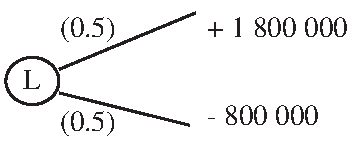
\includegraphics[scale=1.0]{figurer/fig16_6.pdf} 
\caption{Lotteri}
	\label{fig:lotteri2}
\end{figure}
\noindent La oss studere lotteriet $L$ i Figur~\ref{fig:lotteri2}, hvor forventet verdi er 
\[   1\;800\;000 \cdot 0.5 +(-800\;000)\cdot 0.5 = +500\;000    \]
Anta at beslutningstakeren blir tilbudt et fast beløp som erstatning
for lotteriet.  En beslutningstaker som bruker forventningsverdier
som kriterium er indifferent mellom lotteriet og et sikkert 
beløp på 500 000, men villig til å selge lotteriet straks
det tilbudte beløp overskrider 500 000.  En beslutningstaker som har 
sterk aversjon mot posisjonen $-$800 000, vil trolig være villig til å
godta et lavere beløp for å bli fritatt for den risiko lotteriet
innebærer.  Kan hende han er villig til å selge lotteriet for 
ethvert beløp større enn 300 000, men beholde lotteriet for alle beløp
mindre enn 300 000.  I så fall sier vi at beslutningstakerens 
sikkerhetsekvivalent for lotteriet er lik 300 000.  Sikkerhetsekvivalenten
blir et presist mål for beslutningstakerens holdning til den risiko
lotteriet innebærer.  Jo høyere sikkerhetsekvivalenten er, desto
mer risikovillig er beslutningstakeren.

For å kunne bringe beslutningstakerens holdning til risiko inn i 
analysen, må vi ved hver lotteriforgrening i beslutningstreet,
istedenfor forventningsverdien, notere foretakets sikkerhetsekvivalent for
lotteriet.  Analysen forgår da i prinsippet slik:

\begin{enumerate}
\item Beregn foretakets status ved hvert av endepunktene av treet.
\item Beregn systematisk verdien av alle forgreningspunkter ved å
      starte i endepunktene som gis verdi lik status, og gå så
      baklengs i treet til roten.  Hver lotteriforgrening gis en verdi lik
      foretakets sikkerhetsekvivalent, mens hver beslutningsforgrening
      får verdien til den gren som har størst verdi. Denne gren 
      beholdes, de andre strykes.
\item Et optimalt handlingsprogram finnes ved å starte ved roten, og
      følge de grener som ikke er strøket ut.
\end {enumerate}
Ovenfor har vi antatt at sannsynlighetene for de ulike utfall av lotteriet
er gitte, vi har bevisst skjøvet under teppet at det også er 
problematisk å evaluere disse sannsynlighetene.  I praksis vil som 
regel lotteriet $L$ ovenfor fortone seg som i Figur~\ref{fig:lotteri3},

\begin{figure}[ht]
\centering
	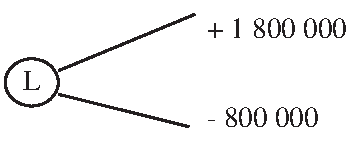
\includegraphics[scale=1.0]{figurer/fig16_7.pdf} 
\caption{Lotteri}
	\label{fig:lotteri3}
\end{figure}
\noindent dvs. uten objektive sannsynligheter for hvert av utfallene. Ønsker 
beslutningstakeren å gjøre en beslutningstreanalyse, må han
være villig til å fastsette sin sikkerhetsekvivalent også for
lotterier hvor sannsynlighetene ikke er objektivt gitt.  Han må da
foreta en simultan vurdering av sjansene for de ulike utfall og deres 
konsekvenser.  Vurderingen vil nødvendigvis måtte bli mer eller
mindre subjektiv, og det endelige valg av sikkerhetsekvivalent vil
representere en beslutning fra beslutningstakerens side.  Analysen foregår
så i prinsippet som ovenfor.

I praksis er som regel et beslutningstre omfattende og komplisert, og for
beslutningstakeren kan det fortone seg problematisk, tidkrevende, uvant
og frustrerende å måtte ta stilling til en rekke fiktive 
lotterier, ofte av sammensatt natur, hvor både vurdering av 
usikkerhet og konsekvenser skal komme til uttrykk.  Heri ligger også
faren for at beslutningstakeren gjør seg skyldig i inkonsistente
vurderinger.  For å redusere disse problemer kan det være
hensiktsmessig å skille beslutningstakerens vurdering av usikkerhet
og konsekvenser.  Videre vil det være ønskelig om 
beslutningstakerens holdning til konsekvenser er tilstrekkelig klarlagt
på forhånd, slik at denne kan brukes ved vurderingen av ethvert
lotteri som inngår i treet.


\section{Preferanseindeks: Nytte}

En beslutningstaker skal ta stilling til et eller flere prosjekter, der det i 
hvert kan inngå både egne og andres beslutninger samt usikre utfall som
gjensidig avhenger av hverandre. Hver situasjon med usikkert utfall vil vi 
kalle et lotteri med gevinster, men gevinstene kan godt selv være et 
lotteri. 

Når vi nedenfor bruker betegnelsen prospekt, kan det bety
en gevinst (g), et lotteri (L) eller et helt prosjekt (P) som i forrige
avsnitt. Dersom 
beslutningstakeren foretrekker prospekt $a$ framfor prospekt $b$ skriver
vi $a\succ b$.  Dersom beslutningstakeren er indifferent mellom
prospektene $a$ og $b$ skriver vi $a\sim b$.  Vi antar at
beslutningstakeren, dersom han får seg forelagt to prospekter
$a$ og $b$, alltid er i stand til å avgjøre om $a\succ b$,
$a\sim b$ eller $b\succ a$.  

Vi kunne ønske oss en preferanseindeks $\pi$ med egenskapen
\[ \mbox{\ \ \ } a\succ b \Longleftrightarrow \pi (a) > \pi (b) \]
slik at ulike prospekter kan rangeres etter deres ``beregnede" preferanse,
og at denne indeksen tillater bruk av de vanlige regne\-regler for sannsynlighet 
og forventning. Dette er mulig dersom beslutnings\-takeren
oppfyller følgende prinsipper for konsistent adferd:

%\begin{center} 
\framebox[10cm]{
\begin{minipage}{9cm}\rule{0cm}{0.5cm}
\noindent {\bf Transitivitet:}\\  La $a, b$ og $c$ være tre
alternative prospekter.
\begin{enumerate}
\item Dersom $a\sim b$ og $b\sim c$, så må $a\sim c$
\item Dersom $a\succ b$ og $b\succ c$, så må $a\succ c$
\item Dersom $a\succ b$ og $b\sim c$, så må $a\succ c$
\end{enumerate}
\noindent {\bf Substitusjon:} 
\\ Gitt et lotteri $L$, og la $L$'
være det lotteri vi får ved å erstatte en av gevinstene $g$
med en annen gevinst $g$'.
\begin{center}
   Dersom $g\sim g$'  så må $L\sim L$' 
\end{center}%\\
\mbox{} 
\end{minipage}
%\end{center}
} 
Det kan vises at en beslutningstaker som oppfyller
disse to adferdsantakelsene vil oppføre seg som om det var tilordnet
sannsynligheter til  alle utfall og preferanser til  alle gevinster
som omfattes av prospektene, slik at preferansen for
de enkelte lotterier som inngår er forventet preferanse for gevinstene.
Videre er helheten logisk konsistent, dvs at de vanlige 
regne\-reglene for sannsynligheter og forventninger gjelder for alle
sammensatte lotterier såvel som hele prosjektet. 

I litteraturen blir prefe\-ranse\-indeksen ofte kalt {\em nyttefunksjonen}.
og resultatet kalles {\em nytteforventningsteoremet}.
Dersom nyttefunksjonen er gitt vil beslutningsproblemet bestå i å
maksimerere forventet nytte.

\begin{figure}[ht]
\centering
	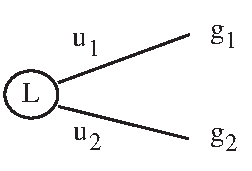
\includegraphics[scale=1.0]{figurer/fig16_8.pdf} 
\caption{Lotteri}
	\label{fig:lotteri4}
\end{figure}
Dette betyr f.eks. at for en konsistent beslutningstaker som står
overfor et lotteri $L$ med to utfall $u_1$ og $u_2$, hvor gevinstene er
henholdsvis $g_1$ og $g_2$ (se Figur~\ref{fig:lotteri4}), så vil
\[  \mbox{\ \ \ } \pi (L)=\pi (g_1)p(u_1) + \pi (g_2)p(u_2)     \]
dvs. nytten av lotteriet $L$ er lik summen av 
nytten for gevinstene veid med de subjektive sannsynligheter
for de respektive utfall eller m.a.o. lik forventet nytte.
Dette kan så holdes opp mot nytten av andre lotterier eller nytten av
en sikker gevinst $g$.

Bestemmelsen av sannsynligheter og preferanser kan i prinsippet reduseres til
beslutninger av følgende to typer:

\begin{enumerate}
\item {\bf Kalibrerende urne:}\\
      Gitt en urne med et stort antall (f.eks. 1000) kuler av ulike farger,
      en farge til hvert
      av de mulige utfall av det lotteri $L$ som er under vurdering.
      Betrakt et alternativt lotteri $L$' som er tilfeldig trekning av en kule
      fra urnen, der gevinsten svarer til fargen på kulen, dvs. samme 
      gevinster som lotteriet $L$.                            
      Blandingsforholdet mellom fargene varieres inntil beslutningstakeren
      er indifferent mellom $L$ og $L$'. Sannsynlighetene for de ulike utfall
      er da gitt ved andelen kuler av de respektive farger.
\item {\bf Referanselotteri:}\\
      Betrakt et lotteri med to monetære referansegevinster $g^+$ og $g^-$, som er
      slik at $g^+\succ g\succ g^-$ for alle aktuelle gevinster $g$.
      Ved vurdering av gevinsten $g$ kan beslutningstakeren bruke en
      kalibrerende urne, f.eks. med $+$ kuler og $-$ kuler. 
      Blandingsforholdet mellom $+$ kuler og $-$ kuler varieres inntil
      beslutningstakeren er indifferent mellom dette lotteriet og gevinsten
      $g$. Preferanseindeks for $g$ er da andelen $+$ kuler.
\end{enumerate}
Det er klart at ethvert lotteri med et endelig antall utfall og tilhørende
gevinster kan ved substitusjon reduseres til et lotteri om de to 
referansegevinstene, der andelene $+$ og $-$ kuler er bestemt ved formelen
ovenfor. Dette er derfor et bevis for nytteforventningsteoremet i dette
tilfellet. Et generelt bevis krever noe mer inngående argumentasjon,
og noen tilleggsantakelser.

Dersom alle aktuelle gevinster er monetære, vil beslutningstakerens
såkalte {\em preferansekurve} være et nyttig hjelpemiddel.
Preferansekurven er preferanseindeksen $\pi(g)$ tegnet som funksjon av 
$g$. I Figur~\ref{fig:prefkurve16} er det tegnet inn tre ulike og karakteristiske 
preferansekurver.

\begin{figure}[ht]
\centering
	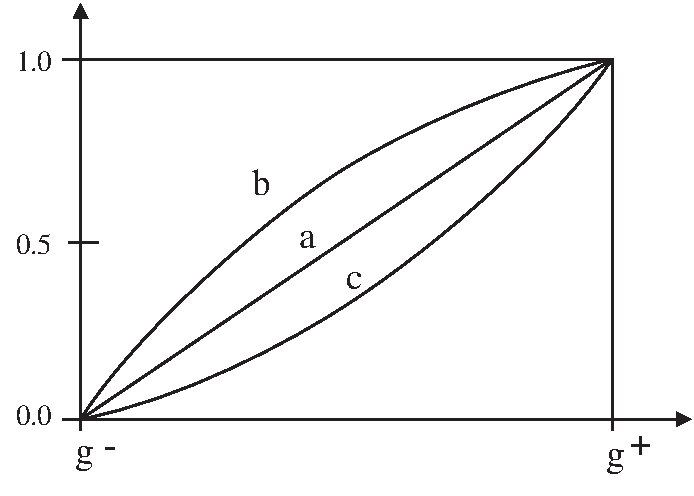
\includegraphics[scale=1.0]{figurer/fig16_16.pdf} 
\caption{Preferansekurver}
	\label{fig:prefkurve16}
\end{figure}

En beslutningstaker som er indifferent mellom ethvert lotteri og dets
forventede gevinst, vil ha preferansekurve lik den rette linje $a$
(lineære preferanser), mens preferansekurvene $b$ og $c$ vil 
representere en beslutningstaker med henholdsvis risikoaversjon og 
risikovilje.  Forsøk å forklare hvorfor!

I de fleste situasjoner kan beslutningstakerens preferansekurve avdekkes
ved at å ta stilling til noen få lotterier, gjerne 50-50 lotterier
(myntkast) fordi slike er lette å forestille seg.  Når så
tilstrekkelig mange punkter på preferansekurven er tegnet inn, trekkes
en glatt kurve gjennom punktene.

Teorien ovenfor kan være nyttig ved beslutningstreanalyse, som kan.
foregå slik

\begin{enumerate}
\item Beslutningstakeren avdekker sine subjektive sannsynligheter for
      utfallene av ethvert lotteri i treet. 
\item Beslutningstakeren avdekker sin nytte for alle endepunktene i treet,
      f.eks ved avlesning på en allerede etablert preferansekurve.
\item Beregn systematisk nytten for alle forgreningspunkter i treet ved å
      starte i endepunktene av treet og arbeide seg baklengs til roten.
      Hver lotteriforgrening får nytte lik forventet nytte av grenene
      basert på de subjektive sannsynlighetene. Hver beslutningsforgrening
      får samme nytte som grenen som har størst nytte, 
      denne gren beholdes, de andre strykes.
\item Et optimalt handlingsprogram finnes ved å starte ved roten, og
      følge de grener som ikke er strøket ut.
\end{enumerate}



Vi tar opp igjen problemstillingen til A/S Elektron fra avsnitt 16.2: 
Beslutningstakeren eva\-luerer først sannsynlighetene
for utfallene av de to lotteriene $L_1$ og $L_2$ 
(hjelpemiddel: kalibrerende urne).  Anta at de subjektive sannsynlighetene
ble som oppgitt tidligere.

Beslutningstakerens avdekker så sin holdning til konsekvensene, 
her uttrykt ved status den 31.des. 1996.  Som hjelpemiddel
bruker vi et refe\-ranse\-lotteri hvor referansegevinstene er valgt lik 
$g^- = -1\;000\;000$ og $g^+ = 2\;000\;000$.  Disse skal tolkes som mulig
status på evalueringsdatoen.  

Beslutningstakeren har tatt stilling til de 4 gevinster -800 000, 0, 
1 000 000 og 1 500 000. Dette ga opphav til følgende nytteverdier:
\begin{eqnarray*}
 \pi (-1\;000\;000) = 0.00,& \pi (-800\;000) = 0.14, & \pi (0)     = 0.50 \\
 \pi (+1\;000\;000) = 0.80,& \pi (+1\;500\;000) = 0.91,& \pi (+2\;000\;000) = 1.00  
\end{eqnarray*}
Disse punktene er tegnet inn i et diagram, og preferansekurven
er tegnet som en glatt kurve gjennom disse, se Figur~\ref{fig:pref_elektron}.
Diagrammet kan være nyttig som korrektiv dersom punktene 
avdekker et mønster som kan tyde på inkonsistens.


\begin{figure}[ht]
\centering
	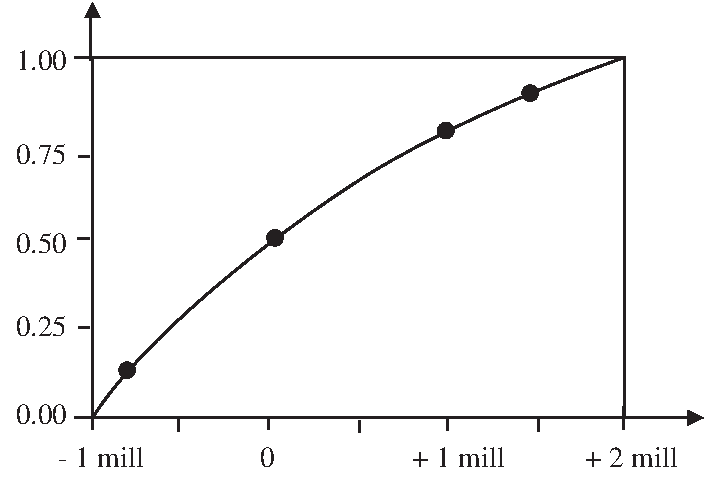
\includegraphics[scale=1.0]{figurer/fig16_19.pdf} 
\caption{Preferansekurve A/S Elektron}
	\label{fig:pref_elektron}
\end{figure}

Vi ser  at beslutningstakeren er indifferent mellom gevinsten 0 og et myntkast
om de to referansegevinstene, og videre at beslutningstakeren
har risikoaversjon, eksempelvis foretrekkes $0$ framfor et myntkast om
gevinstene $-$1 000 000 og +1 000 000, som er et lotteri med forventning {0}.
Illustrer dette i figuren!

\begin{figure}[ht]
\centering
 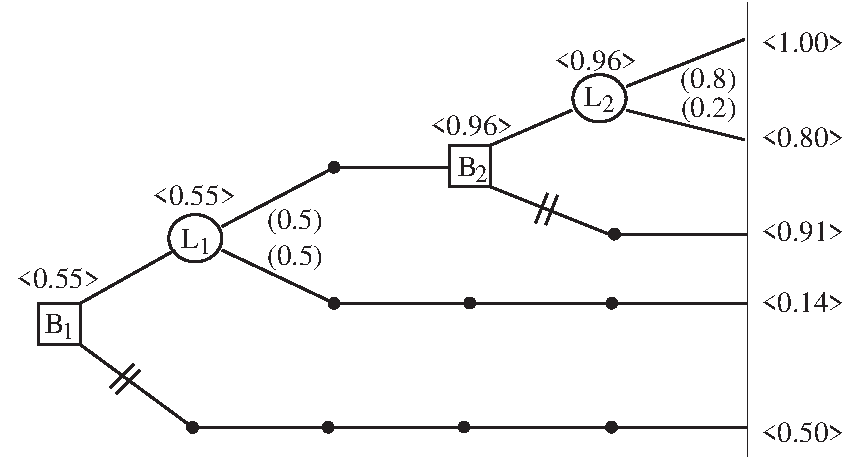
\includegraphics[scale=0.8]{figurer/fig16_20.pdf} 
\caption{Lotteri}
	\label{fig:lotteri5}
\end{figure}

I Figur~\ref{fig:lotteri5} har vi så gjennomført analysen med de funne nytteverdier.
Det overlates til leseren å gjennomgå 
detaljene.  Vi ser at optimalt hand\-lingsprogram for foretaket er 

\begin{itemize}
\item Utvikl prototypen, dersom ordre, produser etter metode 2.
\end{itemize}
Vi ser at nytten for hele prosjektet er 0.55.  Av 
preferansekurven ser vi at dette svarer til sikkerhetsekvivalent på
120 000 kr.  Vi husker at verdien i forventningsverdianalysen var 
500 000 kr., men dersom A/S Elektron har preferanse som uttrykt ovenfor, er
prosjektet verdt bare 120 000 kr.  Vi ser imidlertid at det optimale
handlingsprogrammet er det samme etter begge kriterier.


I vårt enkle eksempel er det bare tre mulige handlingsprogrammer:\\[1mm]
$a_0$: Utvikl ikke prototyp.\\
$a_1$: Utvikl prototyp, dersom ordre, produser etter metode 1.\\
$a_2$: Utvikl prototyp, dersom ordre, produser etter metode 2.\\[1mm]
Hvert av disse handlingsprogrammene vil definere en preferanseindeks i
utgangsposisjonen.  Av Figur~\ref{fig:lotteri5} ser vi at

\[ \pi (a_0)=0.50,\;\;\pi (a_1)=0.525 \mbox{\ \ \ og \ \  }\pi (a_2)=0.55 \]
Det er lett å innse at disse indeksene kan beregnes ved, for hvert 
hand\-lings\-program, å beregne forventet preferanseindeks i 
sluttposisjonen, eksempelvis (se Figur~\ref{fig:apriorifordelinger})

\begin{eqnarray*}
\pi (a_1)&=&p(-800\;000)\pi (-800\;000)+p(0)\pi (0)\\
         & &+p(+1\;000\;000)\pi (+1\;000\;000)+p(+1\;500\;000)\pi (1\;500\;000)\\
         & &+p(+2\;000\;000)\pi (+2\;000\;000)\\
         &=&0.5\cdot 0.14+0\cdot 0.50+0.1\cdot 0.80+0\cdot 0.91+0.4\cdot 1.00
          =0.55
\end{eqnarray*}
Her er benyttet at $p(+1\;000\;000) = 0.5\cdot 0.2 = 0.1$ etter den vanlige
regne\-regel for betingede sannsynligheter.  En analyse av et 
beslutningstre kan derfor utføres ved å beregne preferanseindeksen
for hvert handlingsprogram, og velge det som har størst indeks (nytte).
Dette tilsvarer den analyse\-måten som er beskrevet i avsnitt 16.1.

Noen merknader til slutt: 
I mange bedriftsøkonomiske problemstillinger er det nok slik at 
beslutningstakerens preferanser, i det aktuelle konsekvensområde,
ikke avviker svært mye fra lineære prefe\-ranser.  Det innebærer
at det handlingsprogram som maksimerer forventet fortjeneste som regel
også er det optimale.  En forventningsanalyse vil da kunne raskt gi
en pekepinn på hva som er optimalt, mens den eksakte verdi av 
prosjektet kan avvike betydelig fra forventningsverdien, og kan først
bestemmes ved at preferansene trekkes inn i analysen.  For prosjekter
med stor usikkerhet og med konsekvenser i et stort variasjonsområde, 
hvorav noen kanskje setter foretaket i likviditetsvansker, vil som regel
en forventningsverdianalyse ha liten verdi, preferansene må trekkes
inn i analysen.

I dette avsnittet har vi illustrert den generelle teorien ved et eksempel
hvor alle konsekvensene var monetære.  I praksis har vi svært
ofte beslutningsproblemer hvor også ikke-monetære konsekvenser
inngår, og hvor beslutningstakeren ønsker å ta disse med i 
analysen av problemet.  Det er fullt mulig å trekke slike konsekvenser
inn i en beslutnings\-tre\-ana\-lyse.  Begrepene sikkerhetsekvivalent og
referanselotteri er faktisk nyttige hjelpemidler til å sette en pris
på slike konsekvenser.

\section{Bayesiansk inferens}

Anta at du har en problemstilling som du ønsker å betrakte som
et beslutningsproblem under usikkerhet.  Dersom du er villig til å
følge forutsetninger om konsistent adferd av den typen som er
nevnt innledningsvis i avsnitt 3, så medfører det at din 
holdning til usikkerheten kan la seg representere ved såkalte 
subjektive sannsynligheter som oppfyller de vanlige regneregler for
sannsynligheter som ble utviklet i Kapittel 2 og 4.

Vi vil her ta opp en problemstilling av prinsipiell natur som har 
konsekvenser for statistisk praksis.  Anta at et ``system" kan være
i en av $m$ mulige tilstander ${\theta}_1, {\theta}_2, \ldots, {\theta}_m$,
vi vet bare ikke hvilken tilstand systemet er i.  Situasjonen dreier
seg altså ikke om tilfeldighet, men om uvisshet om tingenes tilstand.
Vi kan illustrere forskjellen med et eksempel.\\

\begin{eksempel}{Falsk mynt?}
I et spill brukes en mynt som kan være
\begin{eqnarray*}
  {\theta}_1 &=&\mbox{rettferdig} \\
  {\theta}_2 &=&\mbox{falsk med kron på begge sider} \\
  {\theta}_3 &=&\mbox{falsk med mynt på begge sider}
\end{eqnarray*}
Anta at du ikke har adgang til å granske mynten nærmere, slik
at du er i villrede om myntens karakter.  Anta at du er i en 
beslutningssituasjon, f.eks. skal velge strategi i et spill hvor
mynten brukes (evt. om du skal delta overhodet).  Tenk deg en rekke
alternative spill der typen av mynt som brukes i hovedspillet bestemmes
ved trekning av en kule fra en urne med kuler av tre farver i 
varierende blandingsforhold.  Når blandingsforholdet er slik at 
du anser dette spill likeverdig med det opprinnelige har vi fått
fastlagt dine subjektive sannsynligheter for de ulike muligheter.  Anta
at resultatet ble

\[ P({\theta}_1)=0.4 \;\;\;\; P({\theta}_2)=0.3 \;\;\;\; P({\theta}_3)=0.3  \]
Vi vil nå se på hvordan disse såkalte 
{\em apriorisannsynlighetene} modifiseres i lys av ny informasjon, f.eks.
ved at du får vite utfallet av en eller flere kast med mynten.  Du
vil antakelig velge følgende modeller for et myntkast for de tre
ulike typer mynter det er tale om 
%\begin{center}
$$
\begin{array}{rcc}
  {\theta}_1: & P(K\mid {\theta}_1)=\frac{1}{2} &
                         P(M\mid {\theta}_1)=\frac{1}{2} \\
 {\theta}_2: & P(K\mid {\theta}_2)=1            & P(M\mid {\theta}_2)=0  \\
  {\theta}_3: & P(K\mid {\theta}_3)=0           & P(M\mid {\theta}_3)=1  
\end{array}
$$
%\end{center}
Vi har her brukt en skrivemåte som antyder at disse sannsynligheter
oppfattes som betingede sannsynligheter gitt type mynt.  Anta at du
får vite at et myntkast med den for deg ukjente mynt ga kron.  Dine
opprinnelige sannsynligheter er nå ikke lenger relevante.  Bayes
lov gir for $i$=1, 2, 3

\[ P({\theta}_i\mid K)=\frac{P({\theta}_i)\cdot P(K\mid {\theta}_i)}{P(K)} \]
hvor
\[ P(K)=P({\theta}_1)\cdot P(K\mid {\theta}_1)+
        P({\theta}_2)\cdot P(K\mid {\theta}_2)+
        P({\theta}_3)\cdot P(K\mid {\theta}_3)  \]
I dette tilfelle blir

\[ P({\theta}_1\mid K)=0.4 \;\;\;\; P({\theta}_2\mid K)=0.6 \;\;\;\;
                     P({\theta}_3\mid K)=0  \]
som kalles {\em aposteriorisannsynligheter} gitt ny informasjon.  Dersom
du får vite at to myntkast ga to kron blir i steden 
aposterisannsynlighetene

\[ P({\theta}_1\mid KK)=0.25 \;\;\;\; P({\theta}_2\mid KK)=0.75 \;\;\;\;
                     P({\theta}_3\mid KK)=0  \]
Det er lett å sjekke at beregning direkte ut fra 
apriorisannsynlighetene og trinnvis beregning ved å modifisere
aposteriorisannsynlighetene etter første kron for en ny kron gir 
samme resultat (se Oppgave~13).
\end{eksempel}

Tankegangen i dette eksemplet kan formuleres generelt slik:  Gitt
$m$ mulige tilstander ${\theta}_1, {\theta}_2, \ldots, {\theta}_m$ og
anta at dine subjektive apriorisannsynligheter for disse er

\[        P({\theta}_i) \;\; ; \;\;    i = 1,2,\ldots, m    \]
For å skaffe informasjon om hvilken $\theta$ som foreligger 
observeres en begivenhet $B$.  Anta at vi etablerer sannsynligheter for det
observerte begivenhet for hver mulig ${\theta}_i$, dvs.

\[        P(B\mid {\theta}_i) \;\; ; \;\;    i = 1,2,\ldots, m    \]
Dine (subjektive) aposteriorisannsynligheter for de $m$ mulige 
tilstandene er da gitt ved Bayes lov

\[ P({\theta}_i\mid B)=\frac{P({\theta}_i)\cdot P(B\mid {\theta}_i)}{P(B)}
    \;\; ; \; \; i=1,2,\ldots , m. \]
Det kunne også være av interesse å ta opp problemstillinger
der ``systemet" kan være i en av et uendelig antall tilstander:\\

\begin{eksempel}{Falsk mynt?}
I et spill brukes en mynt som kan være falsk, la $\theta$ være
sannsynligheten for kron.  Apriori kan $\theta$ være en vilkårlig
verdi i intervallet 0 til 1, dvs. det foreligger et (overtellbart)
uendelig antall muligheter.  Dette kan betraktes som en generalisering
av problemstillingen i Eksempel 2 hvor kun 3 $\theta$-verdier, nemlig
$\frac{1}{2}$, 1 og 0, var apriori mulige. Vi kan nå ønske å gå 
fram på analog måte:  Formulere apriorisannsynligheter for
$\theta$, skaffe informasjon om $\theta$ ved å eksperimentere med
mynten; av dette finne aposteriorisannsynligheter for $\theta$.  Vi ser
at problemstillingen krever omgang med kontinuerlige 
sannsynlighetsfordelinger som fordeler sannsynlighet for $\theta$ i 
intervallet fra 0 til 1. Før vi ser nærmere på dette vender
igjen oppmerksomheten mot inferensproblemet generelt.\\
\end{eksempel}

Vi betraktet i kapitlene 7-15 statistiske inferensproblemer som det å
trekke slutninger om en parameter $\theta$ i en delvis spesifisert modell på
grunnlag av observasjoner, la oss realisert verdi $x$ av en stokastisk 
variabel $X$. La oss anta at modellen kan beskrives ved at 
sannsynlighetsfordelingen til $X$
\[ p(x \mid \theta) \]
er gitt som funkjon av $\theta$, hvor $\theta$ har et gitt mulighetsområde
\footnote{Vi har her brukt symbolene for diskrete fordelinger men, som vi skal
se senere, vil vi anvende analog tankegang i tilfellet med kontinuerlige
fordelinger.}.
Forøvrig antas $\theta$ å være ukjent, og den valgte inferensmetode
tar sikte på å fungere uansett hva den sanne verdi av $\theta$ er. 
De metoder vi har studert tar ikke omsyn til eventuell apriori viten om 
$\theta$, utover eventuelt for å planlegge observasjonsomfanget. 
En mulighet for å innlemme apriori viten om $\theta$ i analysen vil 
være å spesifisere en sannsynlighetsfordeling
\[ p(\theta) \]
som reflekterer ens, mer eller mindre subjektive mening om hvilke 
$\theta$-verdier som er sannsynlige. Denne sannsynlighetsfordelingen kalles
{\em apriorifordelingen} til $\theta$, fordi den oppsummerer vår viten om 
$\theta$ før vi observerer $X$. Vi ønsker å modifisere vår viten 
om $\theta$ i lys av den observerte $x$. Dette kan gjøres ved å bruke 
Bayes lov (se Kapittel 4.2) til å beregne den betingede fordeling for 
$\theta$ gitt $X=x$. Vi får
\[ p(\theta \mid x) = \frac{p(\theta) \cdot p(x \mid \theta)}{p(x)} \]
Her er $p(x)$ den marginale fordeling til $X$ gitt ved
\[ p(x) = \sum_{\theta} p(\theta) \cdot p(x \mid \theta) \]
$p(\theta \mid x)$ kalles {\em aposteriorifordelingen} til $\theta$, fordi den 
oppsummerer vår viten om $\theta$ etterat obsevasjonene foreligger.
Ønsker vi et estimat for $\theta$, kan vi bruke forventningen i 
aposteriori\-fordelingen. En estimator konstruert på denne måten blir
ofte kalt en {\em Bayes estimator}, og denne måten å trekke slutninger
på kalles {\em Bayes inferens}. \\

\begin{eksempel}{Binomisk situasjon}
En leverandør leverer råstoff til en produsent som masseproduserer en
artikkel. Det kan leveres to kvaliteter av råstoffet, og man regner at
kvalitet 1 gir 5\% vrak og kvalitet 2 gir 10\% vrak. Det er gjort avtale med
leverandøren at kvalitet 1 skal leveres og betalingen er deretter. Et parti 
råstoff er mottatt, men mottaker er ikke trygg på at det er av avtalt 
kvalitet. For å klargjøre dette undersøkes $n=10$ ferdige enheter og 
antall vrakede noteres. Anta at antall vrakede $X$ blant de undersøkte
er binomisk fordelt $(n=10, \theta)$, der $\theta$ er enten 0.05 eller 0.10.
Nå er
\[ p(x\mid \theta) = {10\choose x} {\theta}^x (1-\theta)^{10-x} \]
Anta at kjøper apriori tror at sjansen for lureri eller ikke er 
``fifty-fifty". Dette svarer til apriorifordelingen
\begin{center}
\begin{tabular}{c|cc}
 $\theta$    & 0.05 & 0.10 \\ \hline
 $p(\theta)$ & 0.5 & 0.5
\end{tabular}
\end{center}
Bruker vi Bayes formel får vi at aposteriorifordelingen er gitt ved uttrykket

\[ p(\theta \mid x) = 
 \frac{0.5 \cdot {10\choose x} {\theta}^x (1-\theta)^{10-x}}
      {0.5 \cdot {10\choose x} {0.05}^x {0.95}^{10-x}+
       0.5 \cdot {10\choose x} {0.10}^x {0.90}^{10-x}} \]
Anta at observert verdi er $x=2$. Av en tabell over binomiske sannsynligheter
får vi
\[   {10\choose 2} {0.05}^2 {0.95}^8 = 0.746 \mbox{\ \ \ \ og \ \ \ } 
     {10\choose 2} {0.10}^2 {0.90}^8 = 0.2683  \]
Dette gir oss følgende aposteriorisannsynlighter for $\theta$:
\begin{center}
\begin{tabular}{c|cc}
 $\theta$  & 0.05 & 0.10 \\ \hline
 $p(\theta\mid x=2)$& 0.28 & 0.72
\end{tabular}
\end{center}
Det overlates til leseren å sjekke at dersom en isteden hadde valgt 
apriori\-sannsynligheten
\begin{center}
\begin{tabular}{c|cc}
 $\theta$  & 0.05 & 0.10 \\ \hline
 $p(\theta)$& 0.70 & 0.30
\end{tabular}
\end{center}
så ville aposteriorisannsynlighten med det samme observerte resultat bli
\begin{center}
\begin{tabular}{c|cc}
 $\theta$  & 0.05 & 0.10 \\ \hline
 $p(\theta\mid x=2)$& 0.47 & 0.53
\end{tabular}
\end{center}
Aposteriorisannsynligheten kan brukes som grunnlag for å foreta et valg,
påstå at kvalitet 2 er levert eller ikke, eventuelt foreta en (kostbar)
material\-analyse av råstoffet. Hva en bør gjøre vil kunne avhenge av
de kostnadsvurderinger, noe som vi kunne spinne videre på.
\end{eksempel}

Analysemåten vi har illustrert med dette eksemplet er et Bayesiansk
alternativ til hypotesetesting. Vi har også Bayesianske alternativ
til estimering, igjen illustrert med et binomisk eksempel.
En del av den matematikk som trengs for å begrunne metoden fullt ut
ligger utenfor det vi krever av leseren, og på enkelte punkter
nøyer vi oss med å sannsynliggjøre resultatene.\\

\begin{eksempel}{Binomisk situasjon - estimering}
Et firma ønsker å markedsføre et produkt på landsbasis med 
garanti om at ved eventuelle defekter som oppstår innen et år etter 
kjøpedato, vil produktet bli erstattet med et nytt. Før dette gjøres
ønsker firmaet å estimere sjansen $p$ for at en solgt enhet må
erstattes. Dette blir gjort ved å markedsføre produktet i et avgrenset 
område over et kortere tidsrom, f.eks. en måned.
Anta at det i dette tidsrom ble solgt $n$ enheter. Et år senere vil man
observere antall reklamasjoner $X$ som fører til erstatning av produktet.
Under rimelige antakelser er $X$ binomisk fordelt $(n,p)$, dvs.
har punktsannsynlighet
\[ p(x\mid p) = {n\choose x} p^x (1-p)^{n-x} \]
Firmaet har noe forhåndsinformasjon om $p$, bl.a. basert på
laboratorietester av produktet og generell kjennskap til kunders
tilbøyelighet til å kreve sin rett.

I slike situasjoner er det hensiktsmessig å oppsummere  apriori
informasjonen ved å spesifisere en kontinuerlig apriorifordeling for
$p$ over intervallet [0,1], representert ved en sannsynlighetstetthet
med passende form. Bayes lov i denne situasjonen lyder
\[ f(p \mid x) = \frac{f(p)\cdot p(x\mid p)}{p(x)}   \] 
der $p(x)$ er den ubetingende punktsannsynlighet, gitt ved integralet av
telleren mhp. $p$ over intervallet [0,1].
Det er bekvemt å spesifisere en såkalt Betafordeling med parametre 
$(r,s)$ som apriorifordeling for $p$. Denne har formen ($\propto$ betyr
proporsjonal med)
\[  f(p) \propto p^{r-1}(1-p)^{s-1}  \]
Her er $r$ og $s$ er positive tall som kan velges slik at fordelingen får
en form som reflekter apriori kunnskapen. Det kan vises at
\[ \mbox{ Forventningen} = \frac{r}{r+s}  \]
Vi ser at $r=s$ innebærer at forventningen er 1/2.
Noen ulike Betafordelinger med tilhørende forventning er gitt i tabellen
\begin{center}
\begin{tabular}{cc|cc}
 r & s &      f(p)      & Forventning \\ \hline
 1 & 1 &       1        &  1/2        \\
 1 & 2 &    $2(1-p)$    &  1/3        \\
 2 & 1 &    $2p$        &  2/3        \\
 2 & 2 &   $6p(1-p)$    &  1/2        \\
 2 & 3 &  $12p(1-p)^2$  &  2/5        \\
 3 & 2 &  $12p^2(1-p)$  &  3/5        \\
 3 & 3 & $30p^2(1-p)^2$ &  1/2      \\ \hline
\end{tabular}
\end{center}
I figuren er tegnet tettheten for tre kombinasjoner av $(r,s)$.
Leseren kan selv tegne inn noen flere.


\begin{figure}[ht]
\centering
   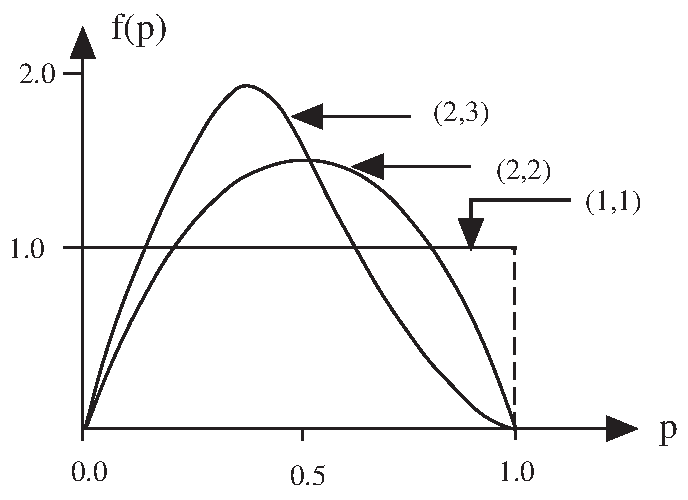
\includegraphics[scale=0.9]{figurer/fig16_x.pdf} 
 \caption{Apriorifordelinger: Beta}
	\label{fig:apriorifordelinger}
\end{figure}
	                   
Vi ser at det er mulig å få frem en rekke ulike fordelingsformer ved 
å velge $r$ og $s$ hensiktsmessig, og i praksis skulle det være mulig
å finne en som avspeiler apriorikunnskapen godt nok.
Figur~\ref{fig:apriorifordelinger} antyder at variansen blir mindre og mindre ettersom $r$ og $s$ 
gjøres større. Er vi derfor nokså sikre på hva $p$ omtrent er,
velges $r$ og $s$ stor, og i samsvar med ens apriori forventning.

Det viser seg at aposteriorifordelingen for $p$ gitt $X=x$ er Betafordelingen
med parametre $(r+x,s+n-x)$. En god gjetning på $p$ er forvent\-ningen i denne
fordelingen som blir
\[   \tilde{p} = \frac{x+r}{n+r+s}   \] 
Dette kalles Bayes-estimatoren for $p$ i den binomiske situsajon
(med Beta-apriorifordeling).

Anta at man finner ut at Betafordelingen med $r=1$ og $s=4$
gir et brukbart uttrykk for apriorikunnskapen om $p$. 
Merk at aprioriforventningen er 0.20, men enhver sannsynlighet er mulig.
Anta videre at det ble solgt $n=100$ enheter, og at etter ett år fikk man
$x=8$ reklamasjoner som medførte erstatning.
Bayes-estimatet for $p$ blir da
\[   \tilde{p} = \frac{8+1}{100+1+4} = \frac{9}{105}=0.076    \] 
dvs. nær det tradisjonelle estimatet, som er andelen erstatninger 0.08.
Merk at med så mange som 100 observasjoner vil disse dominere over den
uttrykte apriorikunnskap. For en mer skråsikker analytiker som innhenter
færre observasjoner vil det være omvendt. Eksempelvis med $r=4$, 
$s=16$ og $n=25$, $x=2$ blir estimatet isteden korrigert fra 0.20 til 0.13, 
selv om aprioriestimatet såvel som observert andel er det samme som ovenfor.
\end{eksempel}



\begin{eksempel}{Målemodellen}
Vi ønsker å estimere forventningen $\mu$ i målemodellen 
på grunnlag av subjektiv forhåndsvurdering og $n$ observasjoner
$X_1,X_2,\ldots, X_n$ med forventning $\mu$ og varians ${\sigma}^2$.
På forhånd forventes $\mu$ å være ${\mu}_0$, og graden
av sikkerhet om dette tenkes uttrykt ved en varians ${\sigma}_0^2$.
Som estimator for $\mu$ kan brukes

\[ \tilde{\mu}=\frac{(n/{\sigma}^2)\bar{X}+(1/{\sigma}_0^2){\mu}_0}
                 {(n/{\sigma}^2)+(1/{\sigma}_0^2)}  \]
dvs. en veid sum av aprioriforventningen og det observerte gjennomsnitt,
med vekter som er omvendt proporsjonale med de respektive varianser.
Denne estimator framkommer dersom vi som apriorifordeling bruker at
$\mu$ er fordelt $N({\mu}_0, {\sigma}_0^2)$ og antar at observasjonene
er uavhengige $N(\mu, {\sigma}^2)$ variable.  Det kan da vises at
aposteriorifordelingen for $\mu$ blir \\$N(\tilde{\mu}, 1/(n/{\sigma}^2 +
1/{\sigma}_0^2))$, slik at $\mu$ er forventningen i aposteriorifordelingen.
Merk at vi må kjenne variansene for å bruke denne estimatoren.
\end{eksempel}

Bruken av Bayes lov er sentral i denne type inferens og statistikere    
som bekjenner seg til denne skolen kalles derfor {\em Bayesianere}
\footnote{Oppkalt etter Thomas Bayes (1702-1761).}.  Det har ofte 
vært faglig uenighet blant statistikere i hvilken utstrekning det er
rimelig å gjøre bruk av Bayesianske metoder.  Hovedinnvendingen
er at siden slik analyse er avhengig av en subjektiv apriorifordeling,
vil to personer kunne trekke forskjellig konklusjon ut fra samme 
observasjoner og den samme modell.  Mange statistikere mener at slik
praksis ikke er tilrådelig, og søker å etablere inferensmetoder
som ikke gir rom for subjektive vurderinger i form av apriorifordelinger,
dvs. slik det ble gjort i Kapittel 7.  Teorien i det kapitlet
representerer klassisk statistisk teori.  Bayesiansk teori er i hovedsak
utviklet senere, selv om id\'{e}en er gammel.

Med Bayesiansk tankegang vil en rekke av de grunnleggende begreper
i klassisk statistisk teori ikke lenger ha noen funksjon, eksempelvis 
forventningsretthet, signifikansnivå, styrke.  Andre begreper får
en helt annen fortolkning, eksempelvis konfidensintervall.

De statistiske problemer som er behandlet i kapitlene 7-15 kan alle
tas opp fra et Bayesiansk synspunkt. Dette krever, selv i de
enklere problemstillingene, matematiske kunnskaper utover det vi har forutsatt.
Imidlertid har de senere års regneteknologi gjort det mulig å
tilrettelegge praktiske tilnærminger, der det meste av teorien kan skjules
for bruker uten særlig risiko for misbruk.	

Ulike skoler statistikere har ofte stått steilt mot hverandre i 
metode\-spørs\-mål og en kilde til uenighet finner vi i 
krysningspunktet mellom objektivitet og subjektivitet.  Debatten er
fremdeles levende, men mange statistikere (iblant dem forfatteren) har
vanskelig for å tro at et felles metodegrunnlag for alle typer
problemer kan finnes, og ser derfor med velvilje på alternativer.
En ting som taler til fordel for Bayesianisme er at det, i hvert fall
i prinsippet, gir en enhetlig ramme for statistiske problemer, en
ramme der forhåndsviten kan og må bringes inn som en integrert
del av analysen.  Bayesianske metoder er vel verdt et nærmere
studium, slike metoder har fått økt popularitet i de senere år,
selv om enkeltes forhåpninger om et Bayesiansk 21. århundre kan 
synes noe optimistisk. 



\section{Oppgaver}
\small
\begin{enumerate}
\item Gitt en situasjon med fem mulige beslutninger og tre mulige 
utfall der gevinstene er gitt ved 
\begin{center}
\begin{tabular}{c|ccccc}
           &\multicolumn{5}{c}{Beslutninger} \\
  Utfall   &  $a_1$ & $a_2$ & $a_3$ & $a_4$ & $a_5$ \\ \hline
   $u_1$   &    1   &   3   &  $-2$ &   4   &   0   \\
   $u_2$   &    0   &   1   &   2   &   2   &   3   \\
   $u_3$   &    1   & $-2$  &   1   & $-2$  & $-1$  \\ \hline
\end{tabular}
\end{center}

\begin{itemize}
\item[(a)] Finn maximin og maximax beslutningen.
\item[(b)] Finnes det noen beslutning som vi kan se bort fra i den videre
           analyse.
\item[(c)] Finn den beslutning som maksimerer forventet gevinst dersom
           sannsynlighetene for de ulike vurderes til 
\begin{center}
\begin{tabular}{c|ccc}
             &  $u_1$ & $u_2$ & $u_3$ \\ \hline
      $p_i$  &   0.1  &  0.6  &  0.3 \\ \hline
\end{tabular}
\end{center}
\end{itemize}

\item
La situasjonen være som i Eksempel 1 med unntak av at tap av goodwill
ved udekket etterspørsel ikke forekommer.  Finn den beslutning som
maksimerer forventet gevinst.
Hva blir forventet gevinst i dette tilfellet?

\item
En bedrift vurderer om de skal utvikle et nytt produkt eller ikke.  
Kostnadene ved å utvikle produktet regnes til 1 mill. kr.
Sannsynligheten for at dette gir et produkt som kan markedsføres vurderes
til 0.7.  Ved eventuell produksjon er to ulike produksjonsvolum aktuelle,
stort eller lite.  Etterspørselen er uviss, her antas for enkelhets
skyld kun to nivåer, høy etterspørsel med sannsynlighet 0.4,
lav med sannsynlighet 0.6.  Netto inntekt i mill. kr. (etter fradrag
av utviklingskostnader) antas å være gitt ved
\begin{center}
\begin{tabular}{l|rr}
           &\multicolumn{2}{c}{Etterspørsel} \\
      Produksjon     &      Høy  &  Lav    \\ \hline
      Stor           &       2.5    & $-0.5$  \\
      Liten          &    $-0.2$    & $-0.3$  \\ \hline
\end{tabular}
\end{center}
\begin{itemize}
\item[(a)] Lag et beslutningstre for problemstillingen der du påfører
           de gitte opplysninger.
\item[(b)] Finn optimalt handlingsprogram dersom bedriften vil maksimere
           forventet inntekt.
\end{itemize}

\item
En bedrift vurderer et prosjekt der største ``gevinst" $g^+$ er 
8 mill. kr., minste gevinst $g^{-}$ er $-$4 mill. kr.  Bedriften anser
en sikker gevinst på 2 mill. kr. som likeverdig med et lotteri der
sannsynlighetene for $g^+$ og $g^{-}$ er henholdsvis 0.8 og 0.2.

\begin{itemize}
\item[(a)] Tegn en preferansekurve som avspeiler dette forhold.
\item[(b)] Anta at den tegnede kurve er bedriftens preferansekurve.
           Hva vil da bedriften foretrekke, sikre 1 mill. kr. eller et 
           lotteri om gevinstene ${-}$1 mill. kr. og 2 mill. kr. med 
           like sannsynligheter?
\item[(c)] Viser den tegnede kurve risikovillighet eller risikoaversjon?
\end{itemize}

\item
Drøft i hvilken grad spørsmålene som ble formulert ved slutten
av avsnitt 16.1 blir besvart i de etterfølgende avsnitt.

\item
Finn aposteriorisannsynlighetene i Eksempel 2 når apriorisannsynlighetene
er
\[  P({\theta}_1) = P({\theta}_2) = P({\theta}_3) = \frac{1}{3}  \]
og vi observerer
\begin{itemize}
\item[(a)] Et myntkast som ga kron.
\item[(b)] To myntkast som begge ga kron.
\item[(c)] To myntkast som ga en kron og en mynt.
\end{itemize}
Løs også oppgaven dersom apriorisannsynlighetene isteden er
\[ P({\theta}_1) = 0.8 \;\;\; P({\theta}_2) = 0.1 \;\;\; P({\theta}_3) = 0.1  \]


\item
(Apriorianalyse)  Mynten i Eksempel 2 blir brukt i et spill der innsatsen
er 100 kroner, mens utbetalingen er 150 kroner dersom du gjetter utfallet
av et kast med mynten.  Anta at de tre mulige mynter apriori anses like
sannsynlige. 

\begin{itemize}
\item[(a)] Tegn et beslutningstre for situasjonen.
\item[(b)] Finn en gjetning som gir størst forventet gevinst.
\item[(c)] Lønner det seg å spille når målsettingen er 
           å maksimere forventet gevinst?
\end{itemize}

\item
(Aposteriorianalyse)  En venn har nettopp spilt spillet i forrige oppgave
og opplyser at mynten viste kron.

\begin{itemize}
\item[(a)] Utnytt denne informasjon til å bygge ut beslutningstreet.
\item[(b)] Finn den gjetning som gir størst forventet gevinst.
\item[(c)] Lønner det seg nå å spille?
\end{itemize}

\item
(Preposteriorianalyse)  En ukjent har nettopp spilt spillet i Oppgave~7
to ganger.  Han tilbyr følgende informasjon for salg:  Betal 20 kroner 
for utfallet av første spill, alternativt betal 30 kroner for utfallet
av begge spill.

\begin{itemize}
\item[(a)] Bygg ut beslutningstreet til å omfatte eventuell kjøp
av informasjon.
\item[(b)] Finn den optimale løsning av problemet.
\item[(c)] Lønner det seg nå å spille?
\item[(d)] Hvor mye vil du være villig til å betale for å
           få perfekt informasjon om myntens karakter?
\end{itemize}

\item
Gjennomfør en alternativ løsning av Oppgave~7, 8 og~9 der vi på
forhånd spesifiserer alle tenkelige handlingsprogrammer og mulige
utfallssekvenser med sine respektive gevinster (jfr. Tabell~\ref{tab:beslutningstabell}).

Hint:  Gjør bruk av regning med betingede sannsynligheter og Bayes lov 
til å finne de nødvendige sannsynligheter.

\item
Et tilbud skal sendes ut til alle medlemmene i en større bokklubb.  To
medarbeidere $A$ og $B$ er satt til å vurdere hvor stor andel som vil
reflektere på tilbudet.  De oppgir følgende subjektive sannsynligheter.
\begin{center}
\begin{tabular}{l|ccc}
Andel som reflekterer   &    0.05  &  0.10  &  0.15  \\ \hline
Sannsynligheter ($A$)     &    0.6   &  0.3   &  0.1   \\
Sannsynligheter ($B$)     &    0.2   &  0.5   &  0.3   \\ \hline
\end{tabular}
\end{center}

Ledelsen velger å tillegge vurderingene til $A$ og $B$ like stor vekt.

\begin{itemize}
\item[(a)] Hvilke sannsynligheter bør i så fall ledelsen legge til
           grunn for beslutning om opplagstall?
\item[(b)] Hva er forventet andel som reflekterer ifølge denne fordelingen.
\item[(c)] Besvar også ($a$) og ($b$) dersom ledelsen tillegger 
           $B$'s vurdering dobbelt så stor vekt som $A$'s.
\end{itemize}

\item
En bedrift har bestilt 100 sekker råstoff, 50 sekker som man vet gir
gjennomgående 5\% defekte artikler (1) og 50 sekker av en noe billigere
kvalitet (2) som gir gjennomgående 10\% defekte.  Ved mottak av 
sekkene går det ikke fram hva som er hva, de er merket $A$ og $B$.
Finn sannsynligheten for at sekker merket $A$ inneholder henholdsvis kvalitet
1 og 2 dersom 

\begin{itemize}
\item[(a)] Bedriften produserer $n$=10 artikler med råstoff fra 
           $A$-sekk og en av disse ble defekt.
\item[(b)] Bedriften deretter produserer $n$=10 artikler med råstoff
           fra $B$-sekk og en av disse ble defekt.
\end{itemize}

\item
$\star$ Vis at dersom informasjon blir tilgjengelig i to porsjoner så gir
trinnvis anvendelse av Bayes lov og direkte anvendelse med all informasjon
samme resultat.  Med symboler, dersom 
\begin{eqnarray*}
 p(\theta ) & \rightarrow & q(\theta )=p(\theta \mid x)
               \rightarrow q(\theta \mid y )\\
 p(\theta ) & \rightarrow & p(\theta \mid x,y)
\end{eqnarray*}

\item
En mynt skal brukes i et spill.  Apriori er enhver verdi av 
kronsannsynligheten $p$ tenkelig.  Anta at vi bruker en apriorifordeling
av den type som er beskrevet i Eksempel 5.  La $X$ være antall kron
i $n$ kast.  Finn Bayes-estimatet for $p$ i følgende situasjoner:

\begin{itemize}
\item[(a)]  $r$ = $s$ = 1,  $n$ =  10,  $X$ = 4
\item[(b)]  $r$ = $s$ = 5,  $n$ =  10,  $X$ = 4
\item[(c)]  $r$ = $s$ = 1,  $n$ = 100,  $X$ = 40
\item[(d)]  $r$ = $s$ = 5,  $n$ = 100,  $X$ = 40
\item[(e)]  $r$ = 4, $s$ = 6, $n$ = 10, $X$ = 5
\end{itemize}

\item
For en gitt produksjonsserie antas strekkstyrken $X$ til et tilfeldig
tau å være normalfordelt $N(\mu, \sigma^2)$.  Kvalitetsnivået
$\mu$ kan variere fra en produksjonsserie til en annen og nivået til
en tilfeldig serie antas apriori å være normalfordelt
$N({\mu}_0, {\sigma}_0^2)$, der ${\mu}_0 = 11.0$ og ${\sigma}_0 = 1.0$.
Av en ny produk\-sjons\-serie velges $n$=4 tau som belastes, deres strekkstyrker
ble 
\begin{center}
\begin{tabular}{ccccc}
         $X_i$:  &  10.6  &  9.7  &  10.1  &  10.8  
\end{tabular}
\end{center}
\begin{itemize}
\item[(a)] Gi et Bayes-estimat for kvalitetsnivået $\mu$ for dette
           partiet dersom $\sigma = 0.4$.
\item[(b)] Finn apriorisannsynligheten og aposteriorisannsynligheten
           for at et tilfeldig valgt tau fra dette partiet tåler en
           belastning på 10.0 kr.

Besvar også oppgaven dersom $\sigma$ isteden er 1.0.
\end{itemize}
\end{enumerate}
\normalsize

